\documentclass[8pt, a4paper]{article}
\usepackage{geometry}
\geometry{total={170mm, 257mm},left=20mm, top=20mm}
\usepackage{graphicx}
\usepackage{hyperref}
\usepackage{listings}

\begin{document}
\setlength \topmargin{-1in}
\title{\textbf{Software Engineering for Distributed and Interactive Systems.}}
\author{\textbf{James Ravenhill}}
\date{}
\maketitle

\section{Introduction} 

The main outcome at the beginning of the project was to create a simple and easy to used piece of software which allows the user to control the buggy without being too complex. Both the hardware and software have been an ongoing development based on feedback given through multiple tests, which a few friends generously took part in. The main objectives of the project are listed below but not limited to:

\begin{itemize}
	\item Reliability - Unreliable connection/data transfer is a disadvantage and creates more problems. This will be explained later in more detail.  
	\item  Multiple methods of communication - By using WiFi, Bluetooth, IR remote and PC. 
	\item Scalability - There should be no software problems while developing the increased load of sensor/capabilities of the buggy. 
	\item Maintainability - comments/documentation is clear to allow future developers to understand the project decisions as they happen. 
	\item Autonomous - The buggy has the ability to move in and out of an autonomous mode.  
\end{itemize}

In this document short snips of the main code will be used in explanations. The main raw code can be found in the submitted documents or on my $\href{https://github.com/james8268/Buggy}{Github}$ account.
 

\section{Design}
In terms of hardware design, the overall aesthetic is not very relevant. This being said, proper cable management and reducing the risk of damaging hardware was a great challenge due to the limited mounting points on the buggy. This challenge was overcome by using blue tac or Velcro to attach the hardware to the buggy without damaging the hardware in the process. 

///////insert two pics of the buggy.  


Below are two images of the main schematic of the buggy and a general communications diagram. 
\begin{figure}[h]
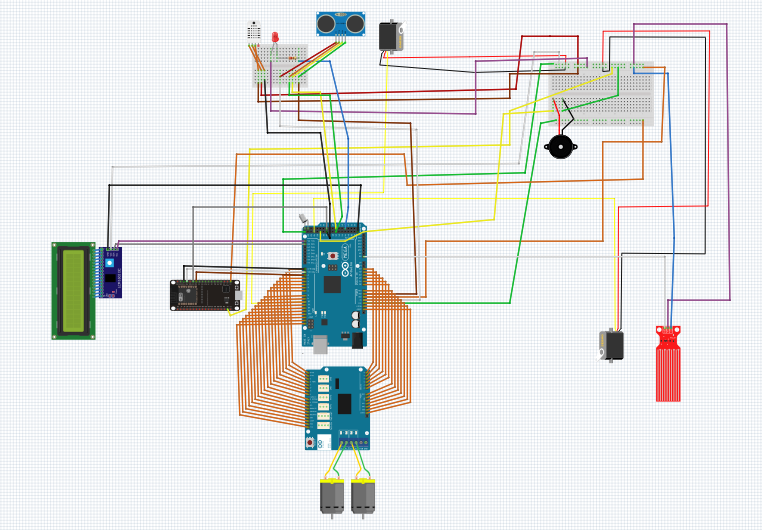
\includegraphics[height=5cm, width=7.0cm]{schematic}
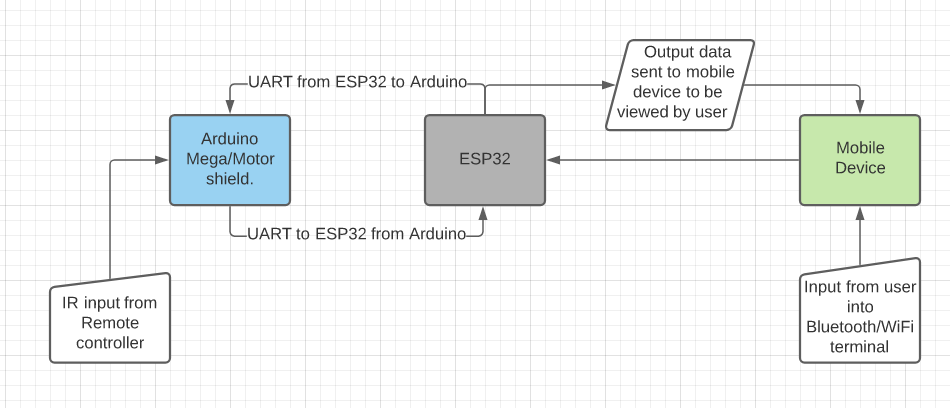
\includegraphics[height=5cm, width=7.0cm]{Arch}
\caption{Left: Schematic of Buggy.}
\caption{Right: general communication graph of the Buggy}
\end{figure}

The software for the Ardunio has been set up into header (.h) files and source code (.cpp) files where they are then called in the main code. There are many benefits to this such as the code is organised and tidy allowing future and current developers to debug with ease, addition of any new code can be easily integrated into the system and the code can be easily maintained. 

\begin{figure}[h]
	
\includegraphics[width=17cm]{tabs}
	\caption{Tabs for Arduino mega main code.}
\end{figure}


The software for the ESP32 comprised of individual sketch files which correspond to the use of WiFi or Bluetooth and for both due to the ESP32 being dual-core. Transmission control protocol (TCP) has been used when using WiFi instead of user diagram protocol (UDP) as is it more reliable, has Flow control so will not overwhelm reciever and has congestion control. A 'handshake' is used to initiate communication and then multiple packets are sent. TCP may not be as fast as UDP but due to the project objectives, reliability is preferred. This being said TCP is slower by a very small margin so is not a large hindrance on the usability of the system. 
 
 
A distributed system is a system which coordinates is actions by communicating between components via passing messages. The example for this project are listed and explained below.

\begin{itemize}
	\item Mobile device-ESP32-Arduino maga: The mobile device communicated to the ESP32 through WiFi (TCP) or Bluetooth, the message that is received by the ESP32 in then passed onto the Arduino mega by universal asynchronous receiver/transmitter (UART). UART is not a communication protocol but is rather a physical circuit where serial data is transmitted and received. This emphasises the reliability factor as no data will be lost over the wired connection. When the Arduino receives a message/command the source code will then action this. If feedback is to then be sent back to the Mobile device it will do so in reverse process, the data will be sent to the ESP32 via UART and then be sent to the mobile device by WiFi/Bluetooth. 
	\item IR signal-Arduino: The IR LED input signal was initially received in the mini-bread board but this cause problems while testing due to high volumes of noise, it was therefore moved directly onto the Arduino mega. This therefore means that the IR remote can by used at the same time as the mobile device. The LCD used the I2C bus to print messages on the screen when temperature, humidity and water sensor readings are requested. 
	\item  PC-Arduino: The PC is connected directly to the Arduino mega and is controlled using the serial monitor. It is very useful for conducting quick simple tests, if new code is added to the software for example. 
	\item ESP32 disconnection feature: When the ESP32 disconnects from the WiFi router or Bluetooth then a signal will be sent to the Arduino mega. When this signal is recieved the buggy will stop, the LCD screen will be cleared and a red LED will light up to alert the user. 
\end{itemize} 

The interactivity between the buggy and the user (besides the obvious mobile device (WiFi/Bluetooth), PC communication and IR remote) consist of the following lower levels of interactiveness:

\begin{itemize}
	\item RFID scanner- This provides security as the RFID tag/card must be presented before any use of the buggy can take place. 
	\item Tilt sensor- This sends a message to the mobile device/PC aswell as sounding an alarm to communicate to the user that the buggy has tipped over due to complex/uneven terrain. 
	\item Disconnection LED- The red LED on the front of the buggy lights up when the WiFi/Bluetooth connection drops.  
	\item Ultrasound sensor- This interacts with its surroundings to gain distance information. This information can then be actioned on accordingly, for example while in an autonomous mode distance information will be used to make decisions and avoid obstacles. 
\end{itemize}
These may seem like simple solutions but they are effective and prove effective during testing. They also provide a level of security to the buggy, the RFID tag can only be added to the source code. 

\section{Implementation}
\begin{figure}[h]
\centering
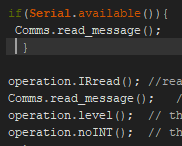
\includegraphics[]{main_loop}
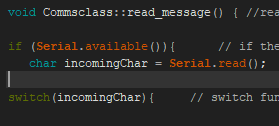
\includegraphics[height=4cm]{read_message}
\caption{Left: Arduino mega main loop}
\caption{Right: Read incoming message}
\end{figure}

Looking at Figure 4 you can see the main loop for the Arduino mega. The commands here are reading the serial monitor when the buggy is connected to the PC as well as the IR remote control reader and the ESP32 reader (this reads messages from the mobile device). Other commands that monitor the tilt sensor and the Wifi/Bluetooth connection are at the bottom of Figure 4. 



3rd Party libraries:
\verb|arduino.h|, \verb|LiquidCrystal_I2C.h|, \verb|IRremote.h|, \verb|Wire.h|, \verb|dht.h|, \verb|SPR.h|, \verb|MFRC522.h|


\section{Testing}

\section{Evaluation}

//// pros and cons of WIFI and bluetooth.
//// limitations to each distributive method.  


\section{Code quality/remarks} ////this may get cut if needed as in more an non written task
////discuss multi and single core methods in a ReadMe file!!!


///Layers- layered system to allow for easy maintenance, ease of updating/developing the system. ADD A DIAGRAM OF THE LAYERS HERE. 


\section{Demonstration}
////film the video and then refer to it for the following subsections


\subsection{Distribution}
///Define what a distributed system is 

\subsection{Interactive}
///Define what an interactive system is

\subsection{Performance}






\section{Conclusion}


\section{Reference Library and appendices}
\subsection{Github account}

\href{https://github.com/james8268/Buggy}{Click here for Github hyper link} 

or copy and paste the URL into your web browser. https://github.com/james8268/Buggy

\listoffigures

\end{document}